\chapter{トランプのデザイン}
\label{0201}
マジシャンやカーディストリーにとってトランプのデザインは重要な要素である.
例えば,マジシャンは図\ref{magic_cards}のようなデザインのトランプをよく利用している.
どちらも上下左右対称であり,白い縁が取られている.
また,煩雑過ぎないデザインが採用されていて,マジシャンの演技を邪魔していないという利点もある.
加えて,同じデザインでカラーバリエーションがあることも重要である.
色が変化する事象は直観的にわかりやすく,インパクトが大きいため,演技の中でバックデザインの色を変えるマジックはよく見られる.

カーディストリーでは,カードを動かす,ディスプレイをするといった特徴から,図\ref{cardistry_cards}のように配色が多いデザインや重心が偏って見えるトランプが採用されている.
また,一般的なトランプのフェイスには,スートや数字,絵札が書かれているが,カーディストリーではスート等を使わないため,フェイスにもバックデザインを施したトランプが登場している.

カジノで使われるトランプもデザインは重要である.
カジノの場合何よりも重要なのがイカサマ防止である.
マーキングという,トランプに黒点などの目印をつけるイカサマがある.
カジノの多くで採用されているのが図\ref{casino}に示したダイアモンドバックというデザインである.
ダイアモンドバックはシンプルな幾何学模様になっており,マーキングがされにくい.
また,ダイアモンドバックのデザインの上下にカジノ名やロゴが描かれているトランプも多く存在する.
カジノでのトランプは消耗品であり,ギャンブルの種類によっては一度のゲームでしか使われない場合もある.
多くのカジノで使われたトランプは一部をカットしたり,インクで塗りつぶしたりして,土産として安価で販売している.
観光客が自身の遊んだカジノの記念品として購入するため,カジノ名などが入ったデザインが採用されている.

また,上記の分野でよくおこなわれる技法にファンとスプレッドがある.
ファンはトランプを扇型に広げる技法であり,スプレッドは横に長く広げる技法である.
トランプによって広げたときの印象が違い,
どちらも右側にカードが重なっていくので,ファンの場合左上に,スプレッドの場合左側に色やデザインがあるとつながって見える.



\begin{figure}[htbp]
    \begin{center}
    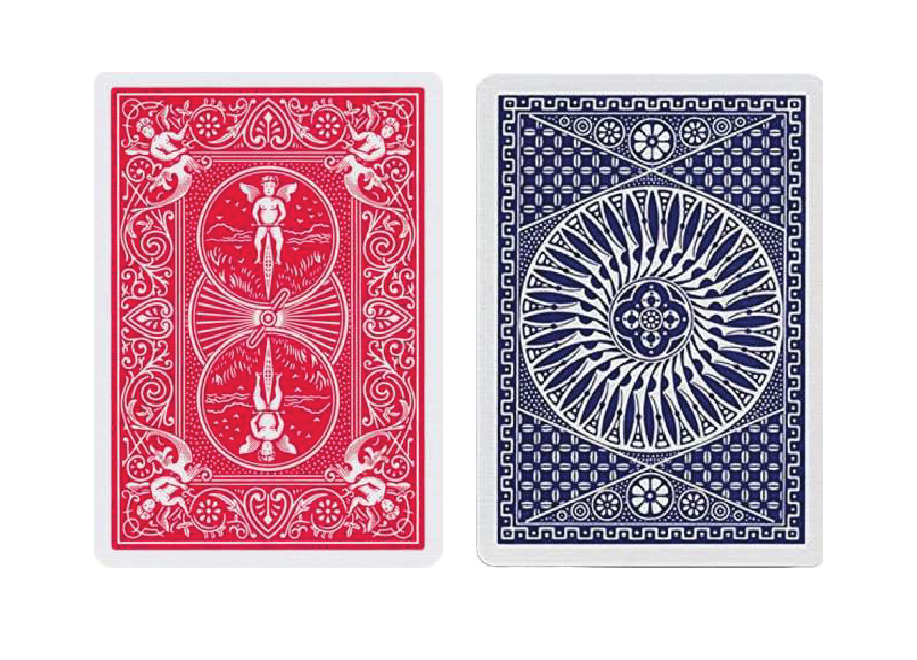
\includegraphics[scale=0.6]{image/playing cards.eps}
    \caption{マジックに向いているトランプのデザイン}
    \label{magic_cards}
    \end{center}
\end{figure}

\begin{figure}[htbp]
    \begin{center}
    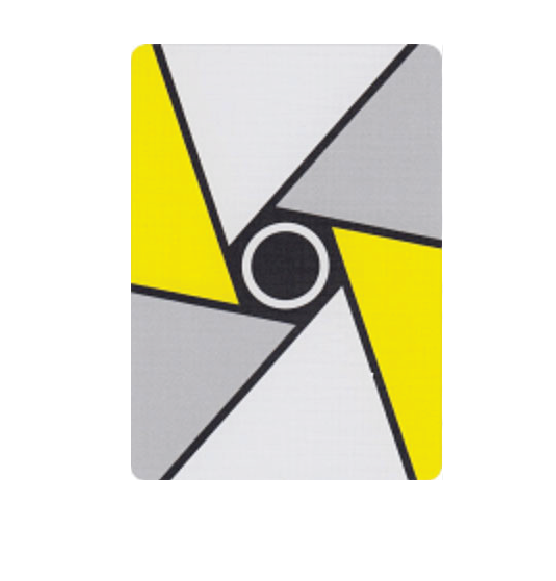
\includegraphics[scale=0.7]{image/cardstry.eps}
    \caption{カーディストリーに向いているトランプ}
    \label{cardistry_cards}
    \end{center}
\end{figure}

\begin{figure}[htbp]
    \begin{center}
    
\includegraphics[scale=0.72]{image/bee.eps}
    \caption{ダイアモンドバック}
    \label{casino}
    \end{center}
\end{figure}
